
\section{Class Introduction}
\subsection{Outline}

\begin{frame}
  \centering
  {\huge
    Week 1 -- Part 1: Class Introduction
  }
\end{frame}

\begin{frame}
  \frametitle{Outline}
  \begin{enumerate}
    \item Outline and goal of the Class
    \item What are programming Challenges?
    \item Initial Example
    \item Class Program
    \item Lecturer Introduction
    \item Extra: ICPC
  \end{enumerate}
\end{frame}

\subsection{Goals of the Class}
\begin{frame}{Class goal: Improve our programming skills!}
\end{frame}

\begin{frame}{Learning Algorithms and Practicing Algorithms}
\end{frame}

\begin{frame}{Automated Judging}
\end{frame}

\begin{frame}{Class Expectations}
\end{frame}

\begin{frame}
  \frametitle{What is this course about?}

  You have learned many programming techniques...\\\hfill \structure{...but can you use them?}

  \begin{block}{Course Objective: Learning by Practice}
    \begin{itemize}
      {\small
    \item Every week: Solve 8 programming challenges;
    \item \structure{Choose} and \structure{implement} the {\bf best algorithm} for each problem;
    \item Be careful with \alert{max time}, and \alert{max memory};
    \item We will discuss algorithms, techniques and tricks;
      }
    \end{itemize}
  \end{block}

  \begin{exampleblock}{Course Goal:}
    Improve programming abilities, techniques and familiarity.
  \end{exampleblock}
\end{frame}

% \begin{frame}
%   \frametitle{Warnings about this class}
%   \begin{alertblock}{1- Heavy Workload}
%     \begin{itemize}
%     \item Starts easy, but hard in the end;
%     \item A few hours/week of homework;
%     \item Lots of debugging;
%
%       \bigskip
%
%     \item Hint: Do your homework early!
%     \end{itemize}
%   \end{alertblock}
%
%   \begin{alertblock}{2- Course Language}
%     \begin{itemize}
%     \item My Japanese is not very good ;-) Let's talk in C++!
%     \item All the course materials are in English;
%     \item You can make your homework in Japanese;
%
%       \bigskip
%
%     \item Practice some English in this course too! :-)
%     \end{itemize}
%   \end{alertblock}
%
% \end{frame}



\subsection{What are Programming Challenges?}
\begin{frame}{What are Programming Challenges}
\end{frame}

% \begin{frame}
%   \frametitle{What is a ``Programming Challenge''?}
%
%   A \structure{puzzle} that you solve by \structure{programming}.
%
%   \bigskip
%
%   Parts of a Programming Challenge:
%   \begin{itemize}
%   \item Description;
%   \item Standard input;
%   \item Standard output;
%   \item Examples;
%   \end{itemize}
%
%   \bigskip
%
%   Task: Write a program that:
%   \begin{itemize}
%     \item Reads the input;
%     \item Prints the \structure{correct} output;
%     \item And nothing else!
%   \end{itemize}
% \end{frame}

% \begin{frame}
%   \frametitle{What is a Programming Challenge? - 2}
%
%   \begin{itemize}
%     \item Program Challenges are good for \structure{Practicing Algorithms}
%     \bigskip
%
%     \item Program Challenges are good for \structure{Rapid Prototyping}
%     \bigskip
%
%     \item Program Challenges are used for \structure{Work Recruiting}
%     \bigskip
%
%     \item Program Challenges are also \structure{very fun puzzles!}
%   \end{itemize}
% \end{frame}
%
% \begin{frame}
%   \frametitle{This course is about Programming Challenges}
%
%   The Goal of this course is \structure{solve programming challenges} to \alert{become better at programming}.
%
%   \vfill
%
%   We will study \structure{algorithms and techniques} that are common in
%   \structure{programming competitions}
% \end{frame}



\begin{frame}{Programming Challenges in the world}
  % School competitions
  % IOI
  % Open Competitions and self-study
  % Recruitment
\end{frame}

\subsection{Example}
\begin{frame}{Example Challenge}
\end{frame}

% \begin{frame}
%   \frametitle{What is a Programming Challenge? - 0}
%
%   Consider a string with $N$ characters chosen from $G,C,T,A$. Ex:
%
%   \begin{center}
%     \emph{\alert<2>{GACA\alert<4>{CATACAG}AT}TA\alert<3>{CATTAC}AGA ... GATACCAGATA}
%   \end{center}
%
%   When you receive pair of indexes $s$ and $e$, calculate the number of "CA"s between $N_s$ and $N_e$. Ex:
%
%   \begin{itemize}
%     \item \only<2->{s = 0, e = 12\hfill 3 repetitions}
%     \item \only<3->{s = 15, e = 20\hfill 1 repetition}
%     \item \only<4>{s = 4, e = 10\hfill 2 repetitions}
%   \end{itemize}
% \end{frame}
%
% \begin{frame}[t]
%   \frametitle{What is a Programming Challenge? - 1}
%
%   \begin{center}
%     \emph{GACACATACAGATTACATTACAGA ... GATACCAGATA}
%     \only<2>{\emph{000112222333333344444555 ... 88888899999}}
%   \end{center}
%
%   \begin{block}{Algorithm Idea 1}
%     Start a counter $c = 0$, loop from $N_s$ to $N_e$,
%     and every time you find "CA", add to the counter.
%     \bigskip
%
%     \alert{Problem: If we have many queries, can we do faster?}
%   \end{block}
%
%   \begin{onlyenv}<2>
%
%   \begin{block}{Algorithm Idea 2}
%     Creat an auxiliary array $A$, that keeps the \alert{Cummulative sum} of "CA"s from $N_0$ to $N_i$.
%
%     \bigskip
%
%     If we want to know the answer, we calculate $A_e - A_s$.
%   \end{block}
%   \end{onlyenv}
% \end{frame}



\subsection{Class Program}
\begin{frame}{Class Topics}
  % Subjects that we are going to tackle in this course
\end{frame}

\begin{frame}{Class Format}
  % movies, pdfs, and exercises
  % more details later
\end{frame}

\subsection{Lecturer Introduction}
\begin{frame}
  \frametitle{About the Lecturer}
  \begin{columns}
    \column{0.4\textwidth}
    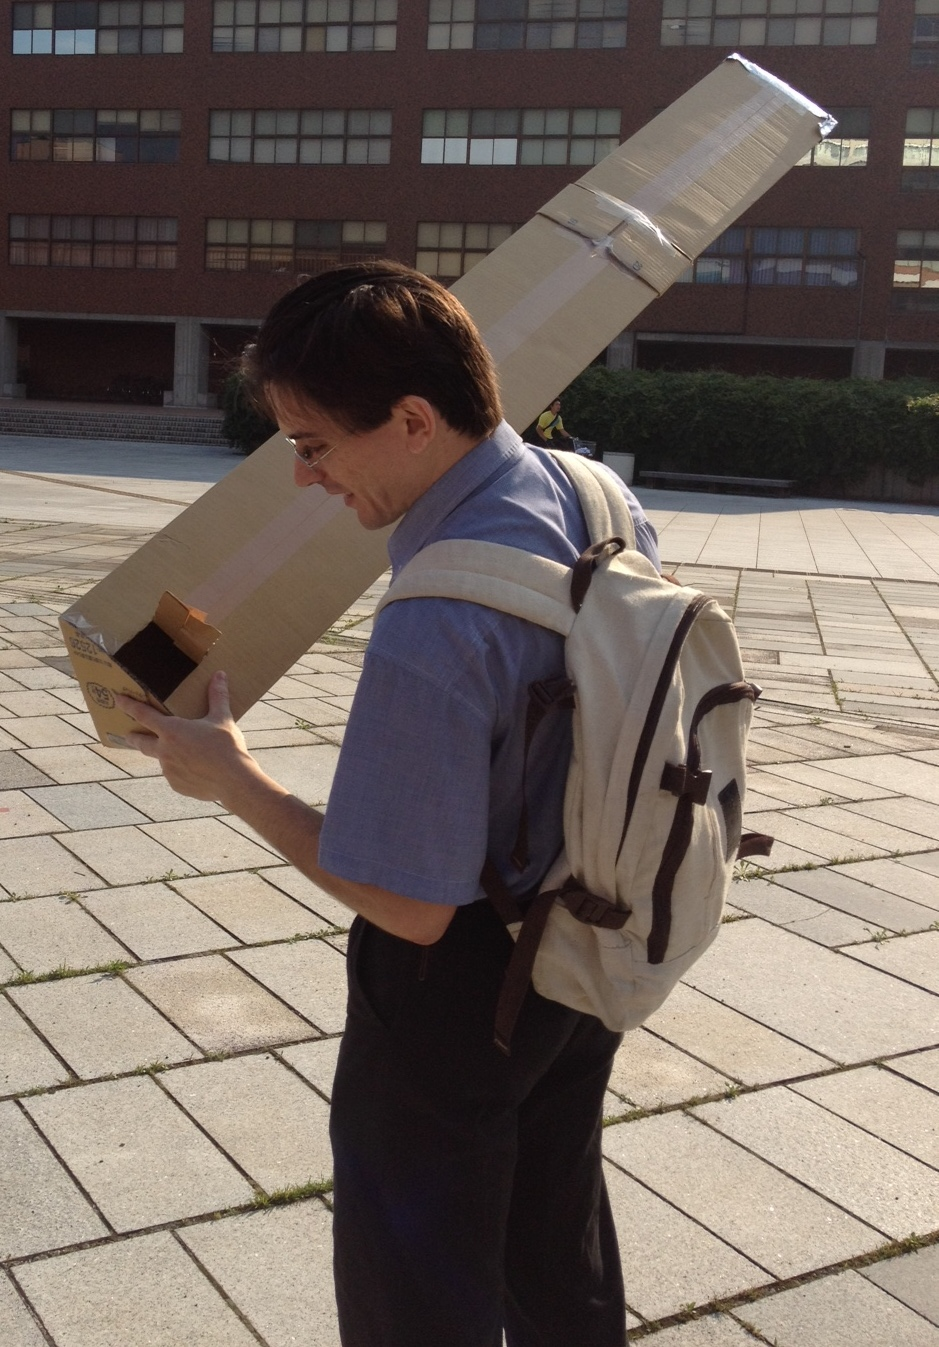
\includegraphics[width=1\textwidth]{../img/pinhole}
    \column{0.6\textwidth}
    {\small
    \begin{itemize}
      \item \structure{Name:} Claus Aranha;
      \item \structure{Country:} Brazil;
      \item \structure{Research:}
      \begin{itemize}
        \item Evolutionary Algorithms;
        \item Artificial Life;
      \end{itemize}
      \item \structure{Hobbies:}
      \begin{itemize}
        \item Programming Games;
        \item Watching Stars;
      \end{itemize}
        \medskip

      \item \structure{webpage:}\\ {\smaller \url{http://conclave.cs.tsukuba.ac.jp}}
    \end{itemize}
    }
  \end{columns}
\end{frame}

\subsection{ICPC}
\begin{frame}{Join the Tsukuba ICPC Team!}
  % What is ICPC?
\end{frame}

\begin{frame}{Join the Tsukuba ICPC Team!}
  % Some ICPC pictures
\end{frame}

\begin{frame}{Join the Tsukuba ICPC Team!}
  % ICPC Requirements, ICPC circle, ICPC calendar
\end{frame}

% \begin{frame}
%   \frametitle{Participate in ICPC!}
%   \begin{columns}
%     \column{0.5\textwidth}
%   \begin{itemize}
%     \item Fun challenges to choose the world champion!
%     \item Teams of 3 people!
%     \item Registration Deadline Early of June!
%   \end{itemize}
%
%   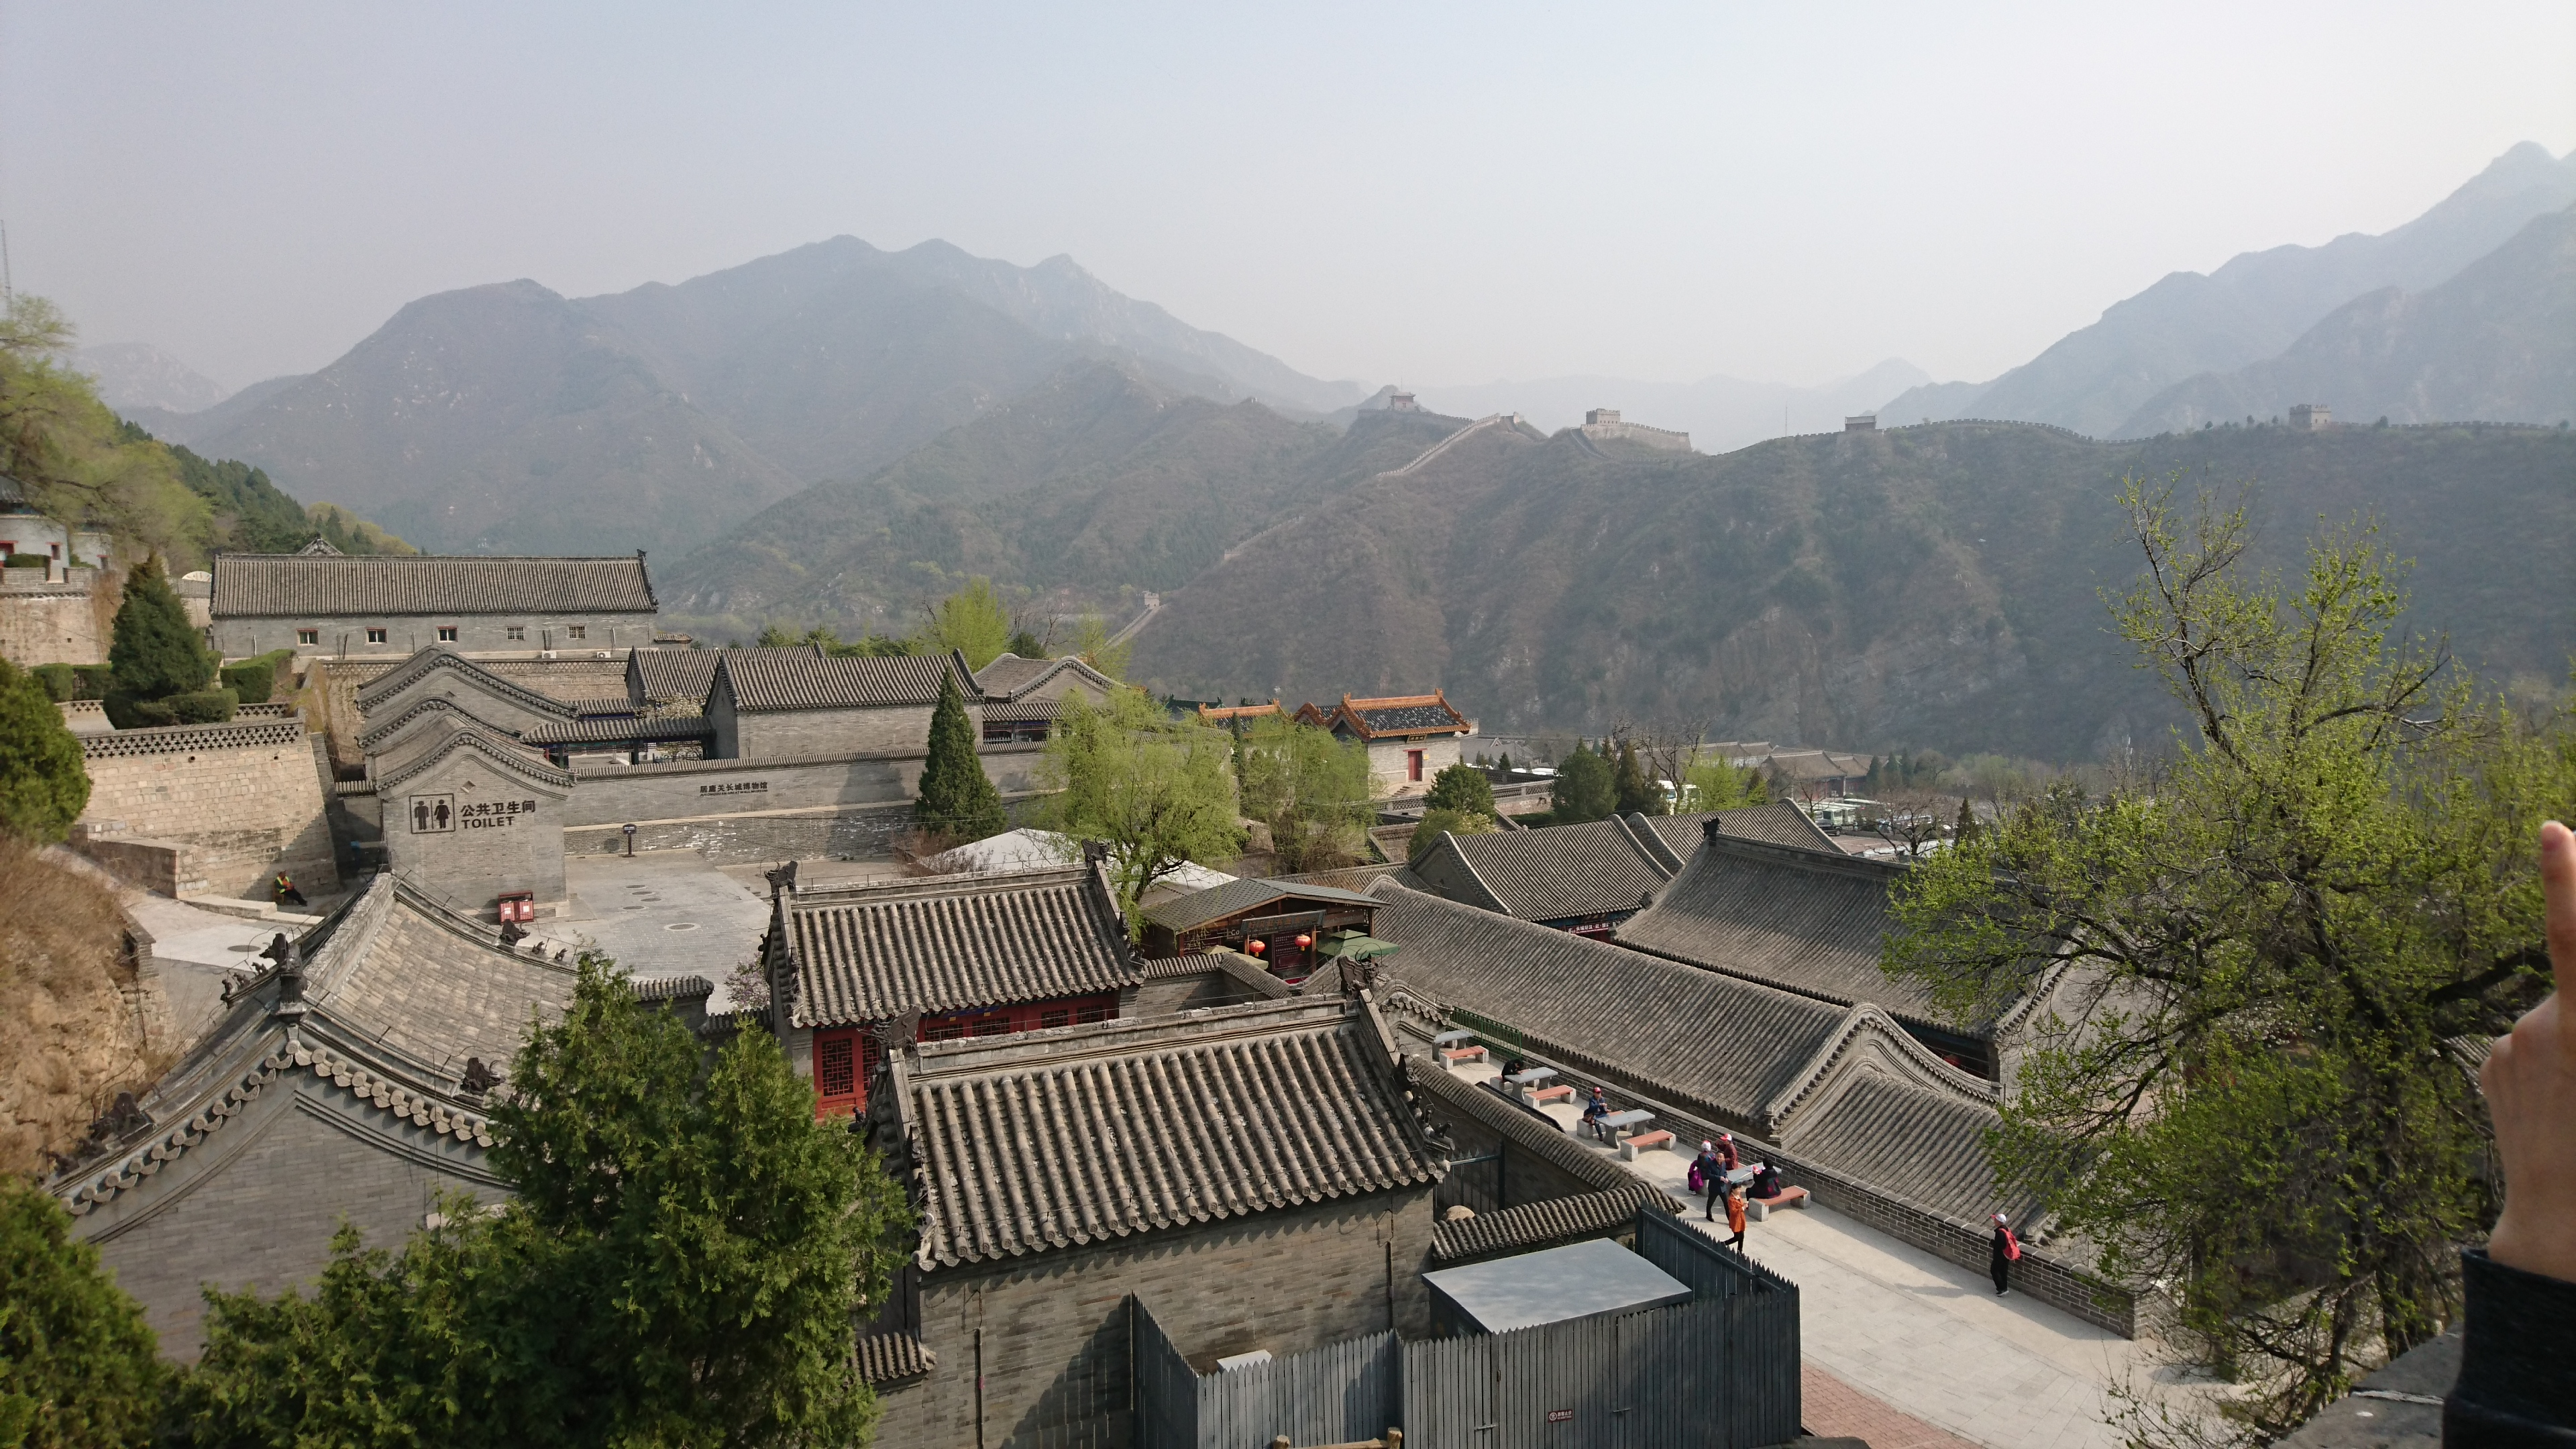
\includegraphics[width=1\textwidth]{icpc/DSC_0171}
%   \column{0.5\textwidth}
%   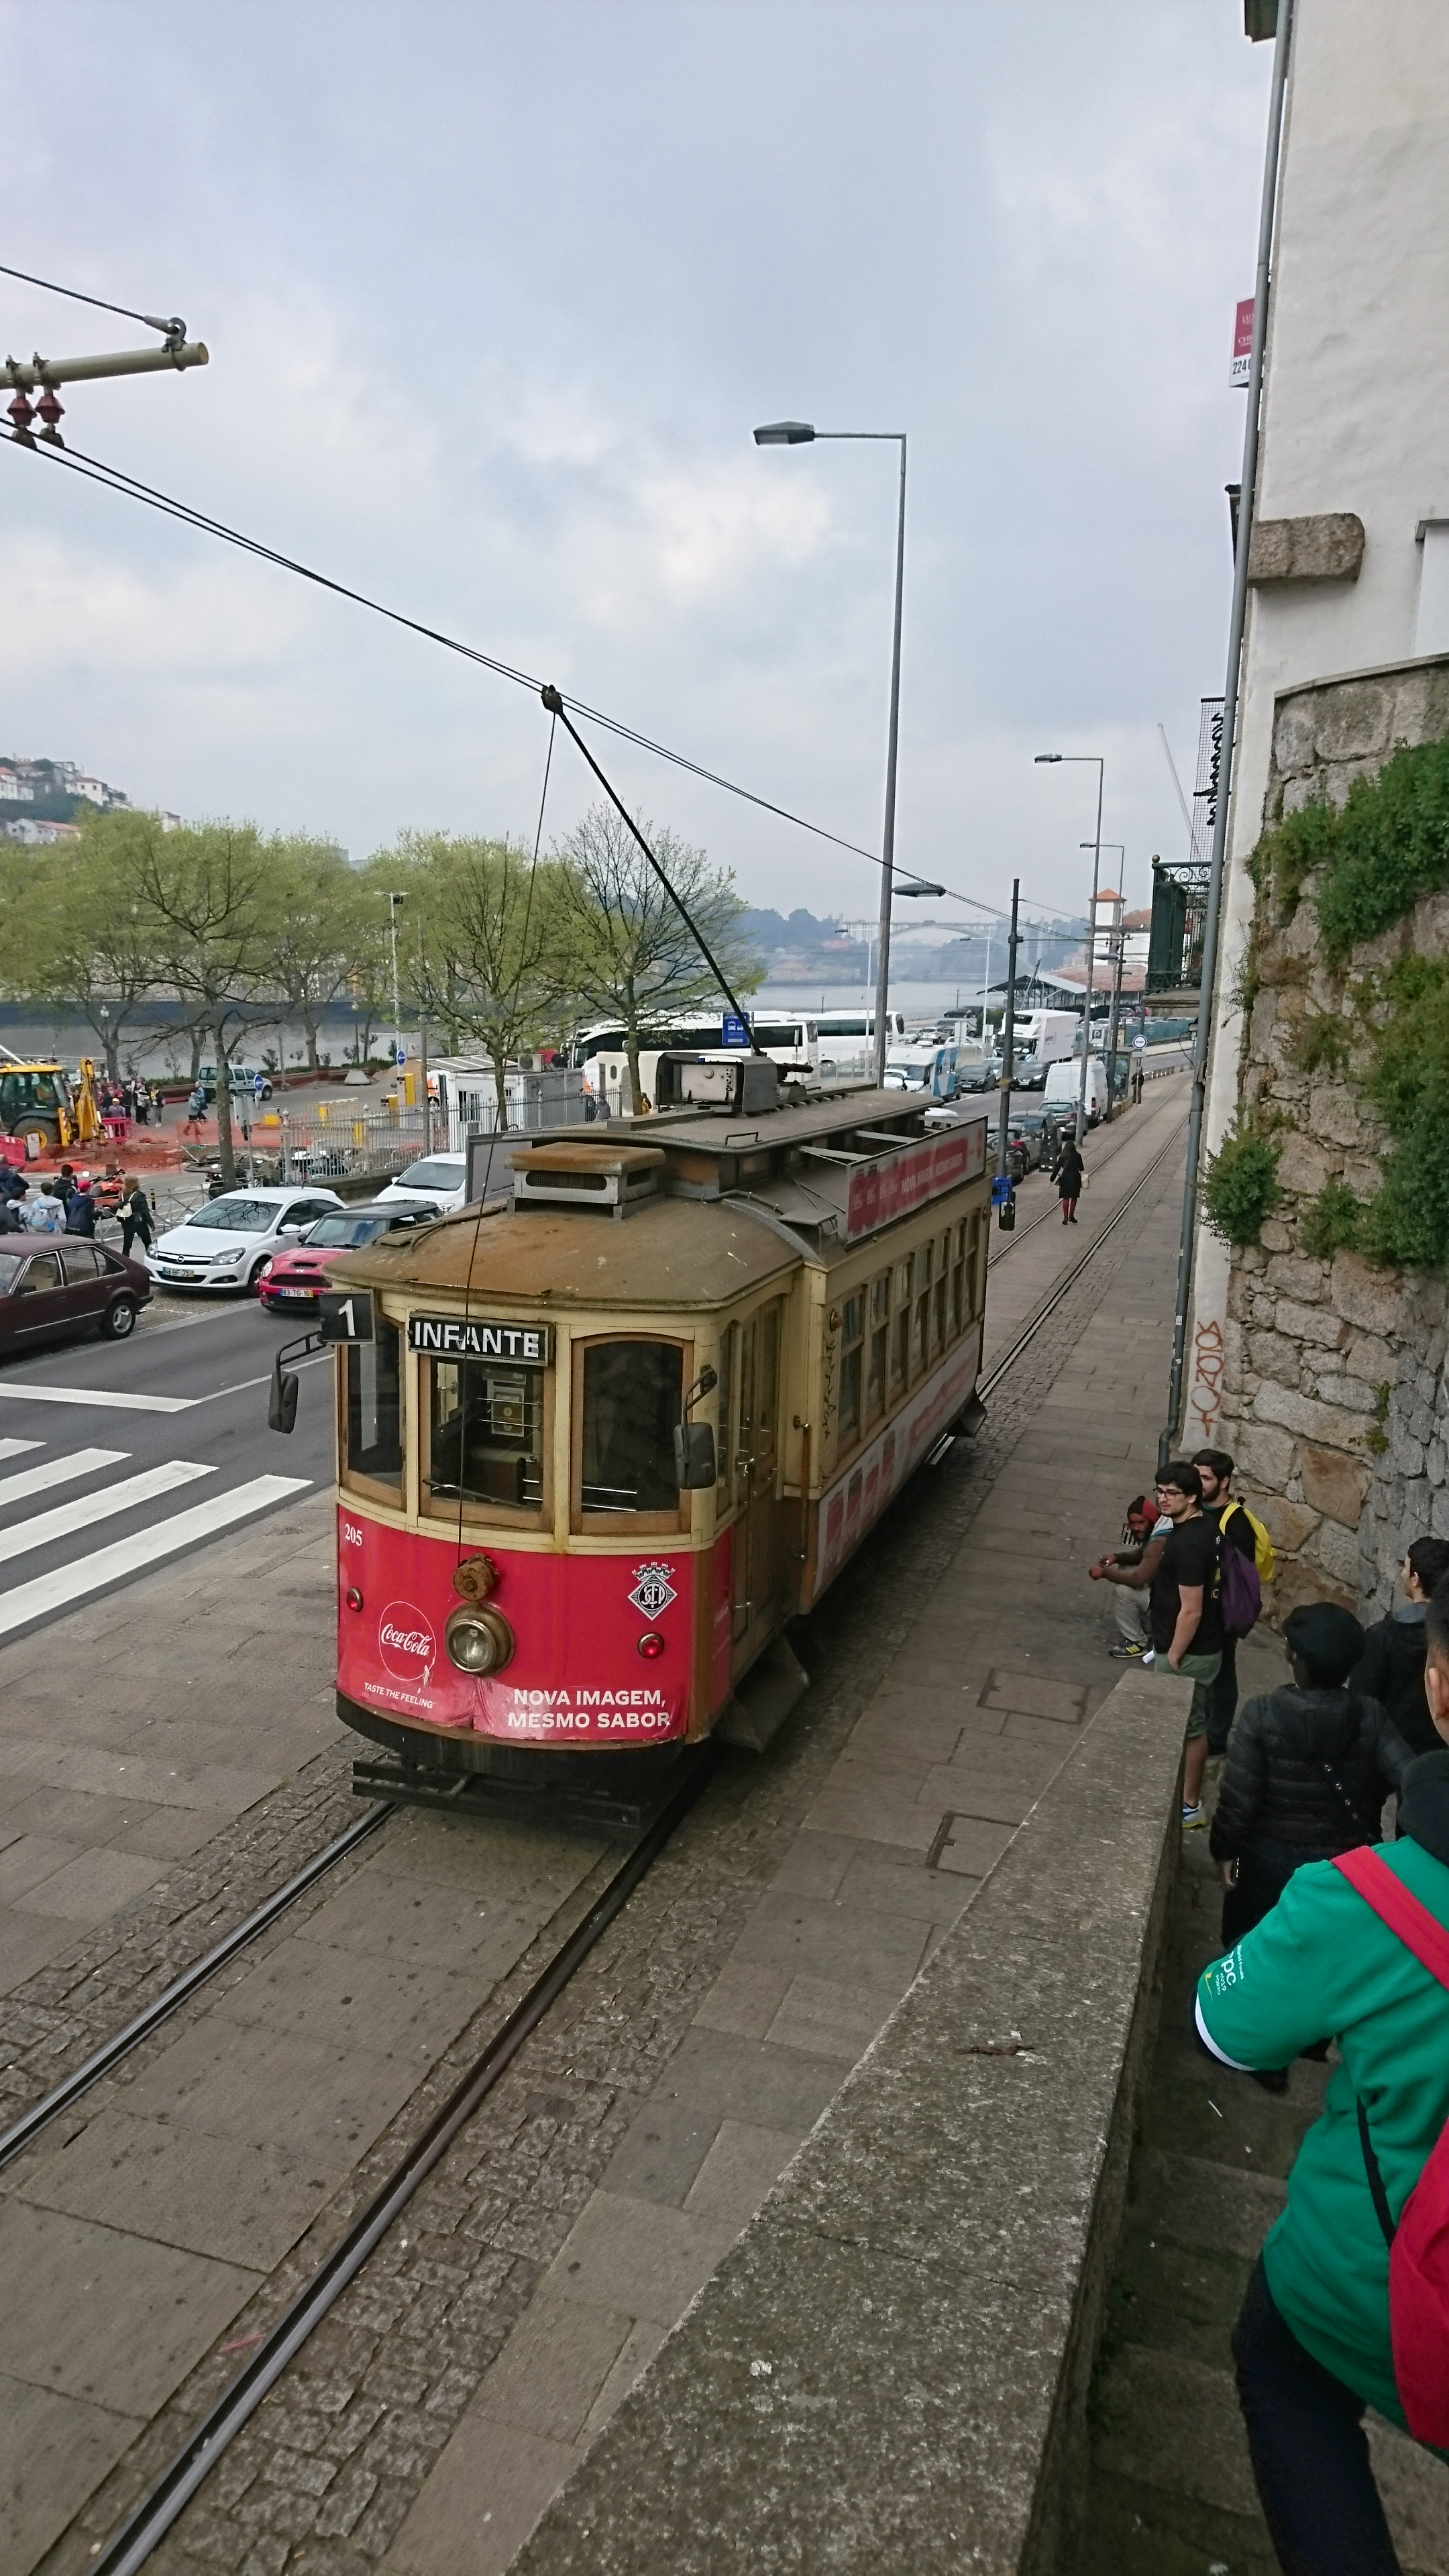
\includegraphics[width=1\textwidth]{icpc/DSC_0677}
% \end{columns}
% \end{frame}



%%%%%%%%%%%%%%%%%%%%%%%%%%%%%%%%%%%%%%%%%%%%%%%%%%%%%%%%%%%%%%%%%%%%%%%%%%%%
